
% < 1 Big Data in der Praxis - Lösungen mit Hadoop, Spark, HBase und Hive. Daten speichern, aufbereiten, visualisieren. 2. erweiterte Auflage, von  Jonas Freiknecht, Stefan Papp, 2018, S
% < 1 https://www.omega.com/en-us/resources/data-loggers
% 0 https://www.researchgate.net/profile/Anne-Ojala/publication/254255682_Eddy_Covariance_A_Practical_Guide_to_Measurement_and_Data_Analysis/links/00b7d51fbaa83999a4000000/Eddy-Covariance-A-Practical-Guide-to-Measurement-and-Data-Analysis.pdf#page=80
Data Logging kann dazu verwendet werden, Code zu debuggen oder große Datenmengen zu speichern, um diese später auszuwerten. Im Allgemeinen ist ein Datalogger ein Instrument, welches Veränderungen unter bestimmten Bedingungen während einer gewissen Zeitspanne aufzeichnet. Ein Datenlogger verwendet häufig Sensoren, um Daten zu sammeln. Anschließend können die Daten ausgelesen, visuell dargestellt und/oder ausgewertet werden. Die Daten, welche von Datenloggern ausgelesen werden, sind meist Druck, Temperatur, Luftfeuchtigkeit, Spannung oder Stromstärke. \cite{DataLogging} 

Die gespeicherten (geloggten) Daten können zum Beispiel dazu verwendet werden, 

\begin{compactitem}
    \item um die Temperatur und die Luftfeuchtigkeit in einem Gebäude zu überprüfen
    \item Information zur Gebäudewartung zur Verfügung zu stellen, dies betrifft das Heizen, die Belüftung, wie die Klimatisierung. Diese ständige Überprüfung der Daten kann den Energieverbrauch reduzieren
    \item die Wachs-Bedingungen von Pflanzen in der Landwirtschaft zu beobachten
    \item die Impfstoff-Lagerung in medizinischen Einrichtungen zu überwachen
    \item die Temperatur von Lebensmittel zu überprüfen
\end{compactitem}
\cite{DataLogging}

Logging bieten eine große Flexibilität und eignet sich gut, um große Datenmengen zu erfassen und auszuwerten. \cite{BigDataBuch}

\subsection{Loggen der Daten in der Firma}
Um die Daten zu loggen, also abzuspeichern, werden diese aus sogenannten Datenpunkten aus der firmentinternen FlexCloud ausgelesen. Diese werden angesprochen und aus ihnen kann dann der aktuelle Wert des Datenpunkts ausgelesen werden, siehe \ref{fig:impl:datenlogging}.
Beispiele für Datenpunkte der Firma FlexSolution, die ausgelesen werden: 

\begin{compactitem}
    \item Daten der Ladestationen
    \item Daten der Photovoltaik-Anlage am Dach
    \item die Temperatur in den Firmengebäuden
    \item Kompressor-Druck von Maschinen
    \item weitere Maschinendaten
\end{compactitem}

\begin{figure}[h t]
    \centering
    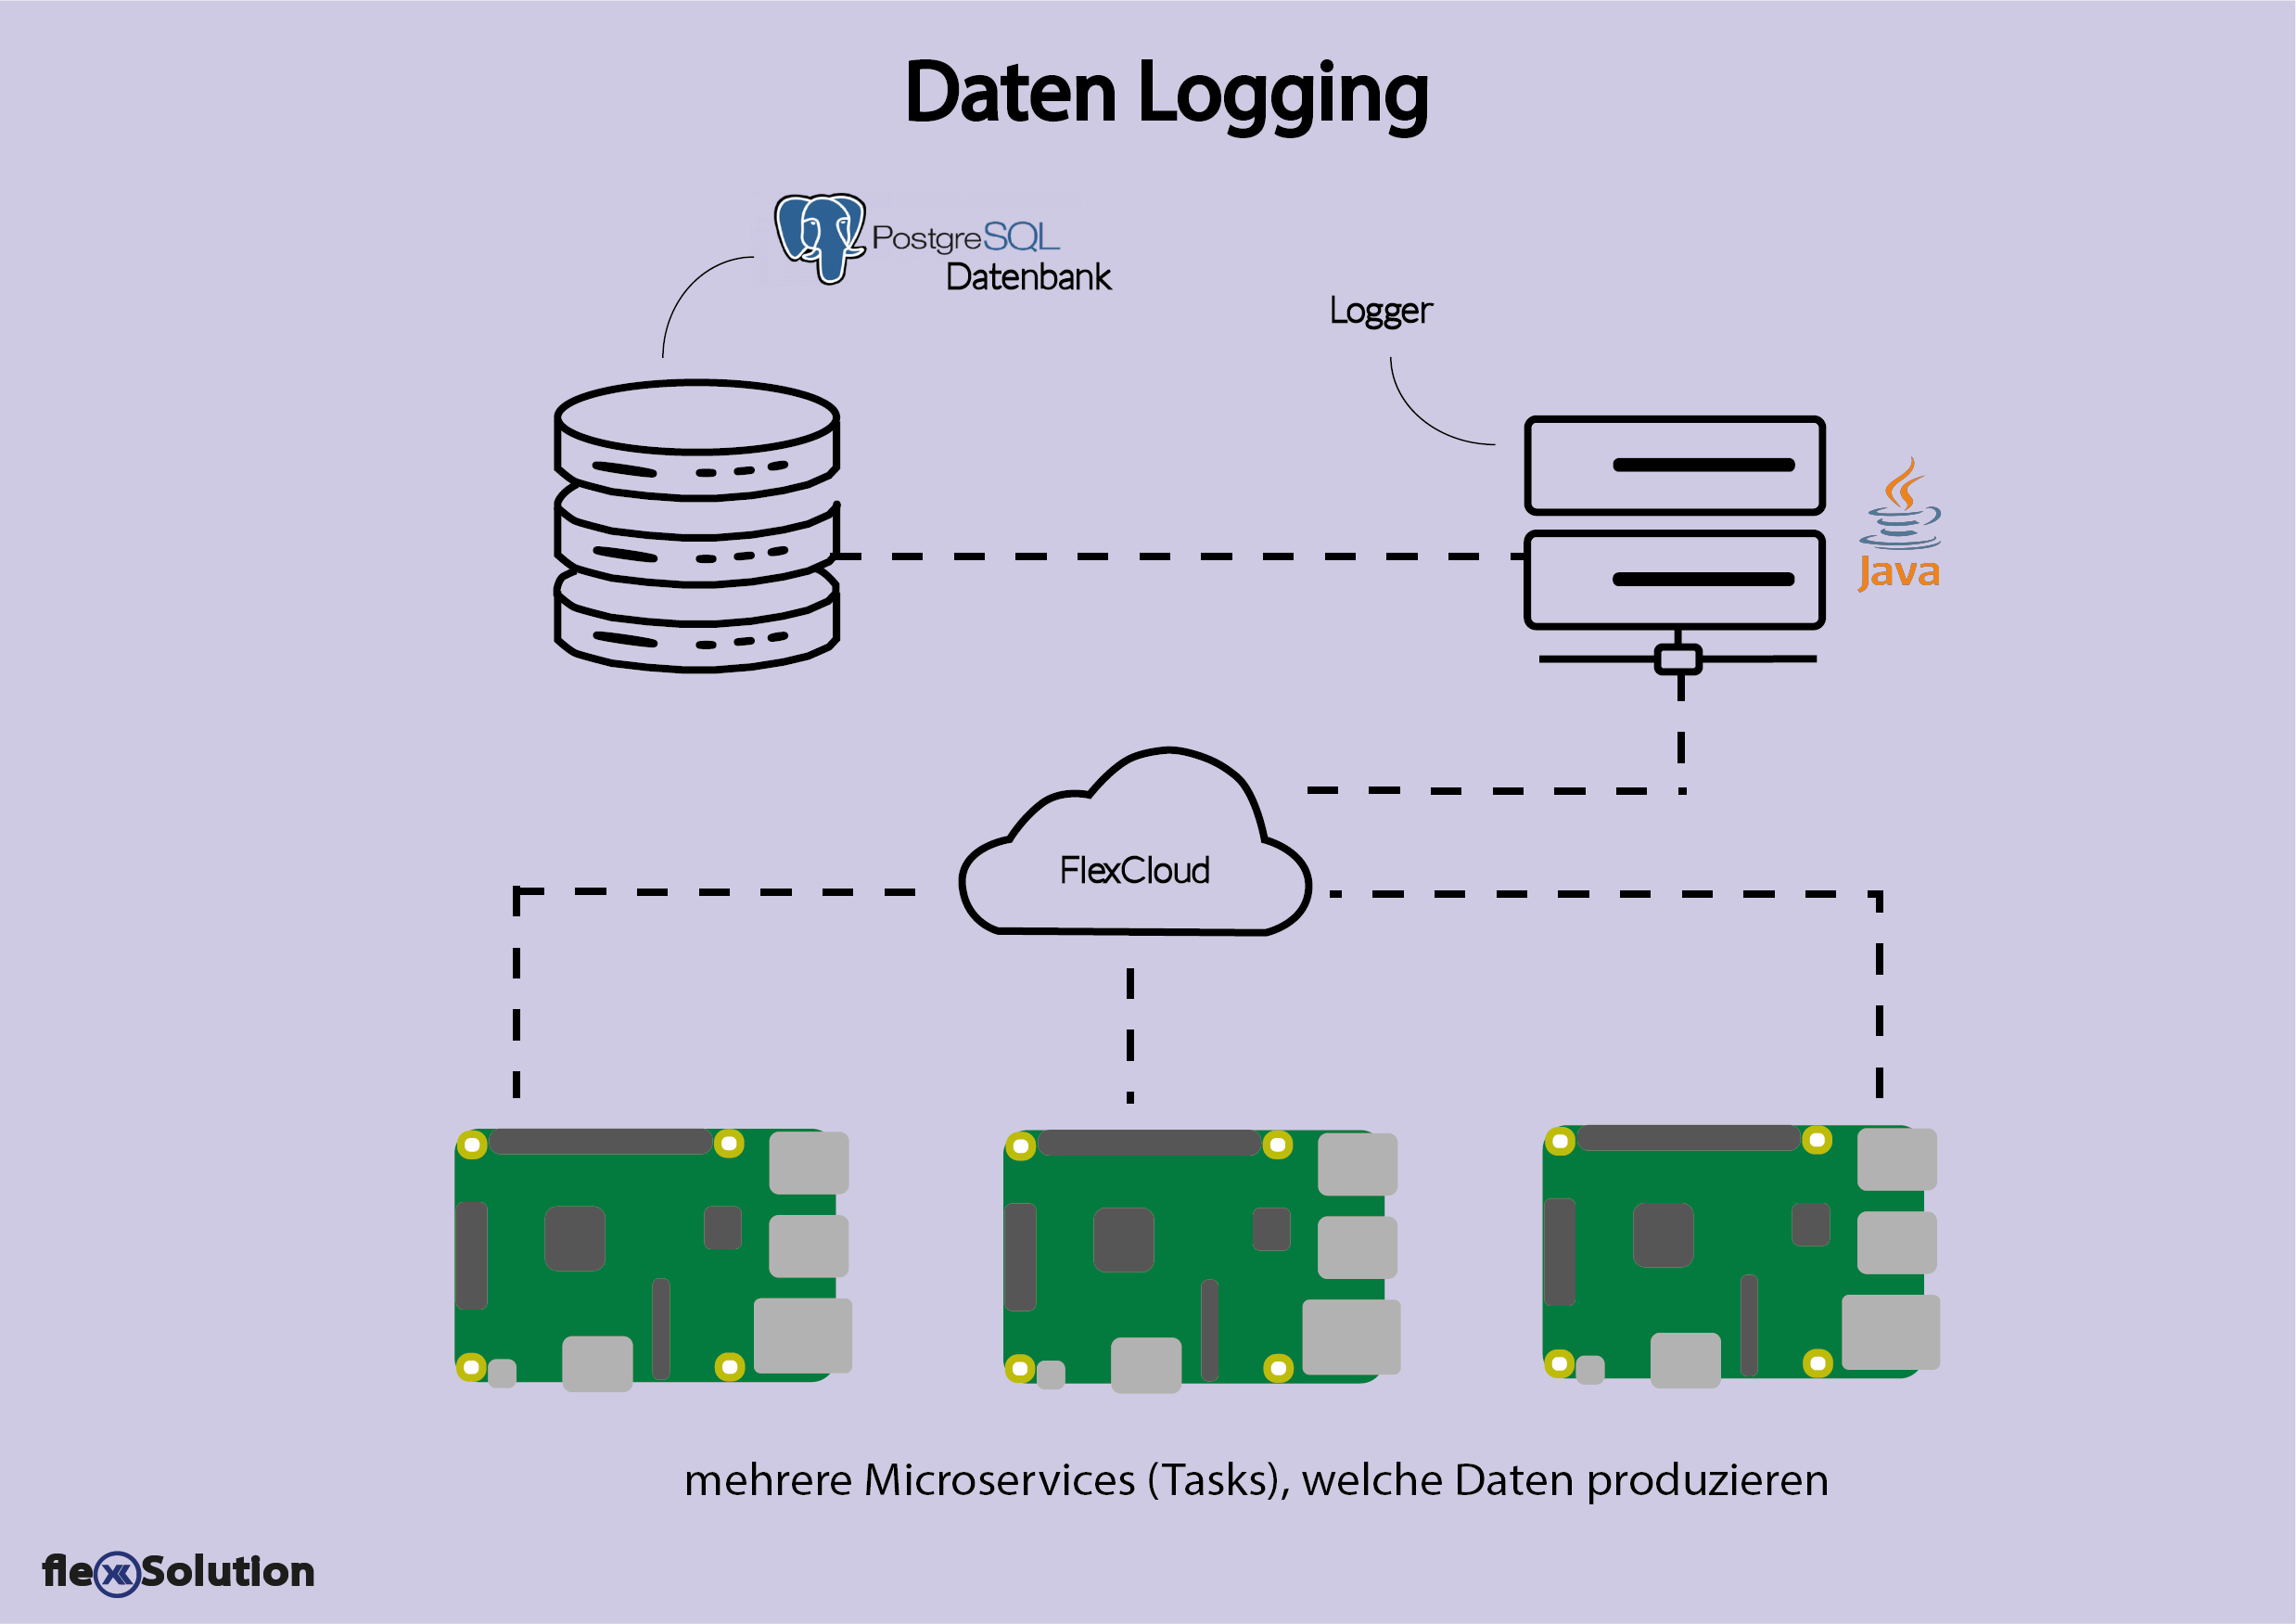
\includegraphics[scale=0.7]{pics/datenlogging.png}
    \caption{Daten Logging}
    \label{fig:impl:datenlogging}
\end{figure}

Das Logging-Programm wird mithilfe des Terminals gestartet. Sobald dieses gestartet wurde, siehe \ref{fig:impl:loggerStart}, werden kontinuierlich Daten in die Datenbank gespeichert. Dies kann in der Ausgabe des Loggers beobachtet werden, siehe \ref{fig:impl:loggerLog}. Um den Logger anschließend zu stoppen, wird ein ähnlicher Command wie beim Starten verwendet, siehe \ref{fig:impl:loggerEnd}.

\begin{figure}[h t]
    \centering
    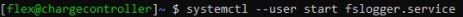
\includegraphics[scale=1.3]{pics/loggerStart.JPG}
    \caption{Logger Programm wird gestartet}
    \label{fig:impl:loggerStart}
\end{figure}

\begin{figure}[h t]
    \centering
    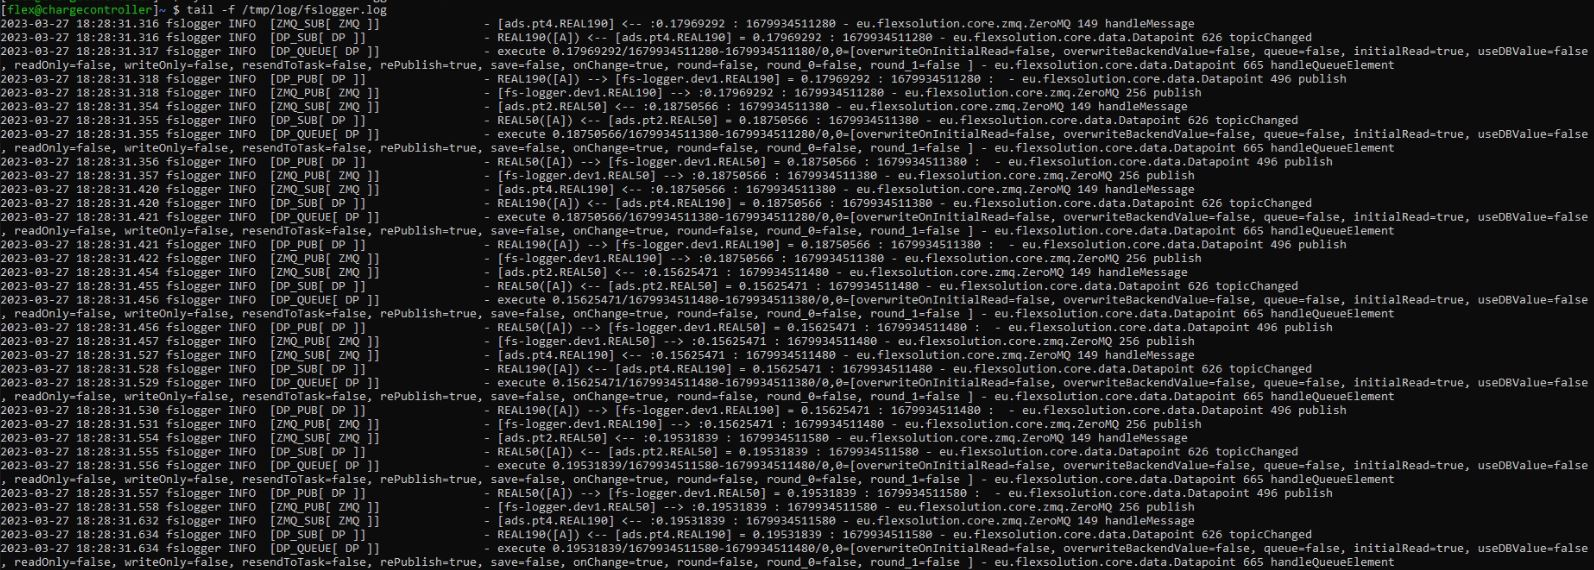
\includegraphics[scale=0.4]{pics/loggerLog.JPG}
    \caption{Ausgabe des Logger Programms}
    \label{fig:impl:loggerLog}
\end{figure}

\begin{figure}[h t]
    \centering
    
\includegraphics[scale=0.75]{pics/loggerEnd2.JPG}
    \caption{Logger Programm wird gestoppt}
    \label{fig:impl:loggerEnd}
\end{figure}

\subsection{Log4J}
% < 1 https://books.google.at/books?hl=de&lr=&id=hZBimlxiyAcC&oi=fnd&pg=PA9&dq=log4j&ots=QiOna081Z6&sig=9h3lwPqN-rm07kAHln-tLSUfgJY&redir_esc=y#v=onepage&q=log4j&f=false The Complete Log4j Manual, von: Ceki Gülcü S15
% < 1 https://logging.apache.org/log4j/2.x/
Log4J ist ein Framework, um Anwendungsmeldungen von Java zu loggen.
Das Design von Log4J konzentriert sich vor allem darauf, schnell, flexibel und leicht verständlich zu sein. Da Logging eine Applikation verlangsamen kann, wird vor allem ein Wert auf die Schnelligkeit gelegt. \cite{log4JBuch} 

Es ist ein populäres Logging-Package für Java. Logging liefert präzise Informationen über den Ablauf einer Applikation. \cite{log4J}


Anwendungen, welche Log4j verwenden, fordern vom LogManager einen Logger mit einem bestimmten Namen an. Der LogManager sucht den entsprechenden LoggerContext und ruft dann dessen Logger ab. 
Wenn erst ein Logger erstellt werden muss, wird er mit der LoggerConfig verknüpft, die entweder 

\begin{compactitem}
    \item[a)] den gleichen Namen wie der Logger, 
    \item[b)] den Namen eines übergeordneten Pakets oder 
    \item[c)] die Stamm-LoggerConfig enthält.
\end{compactitem}

LoggerConfig-Objekte werden aus Logger-Deklarationen in der Konfiguration erstellt. Die LoggerConfig ist mit den Appendern verbunden, welche die LogEvents tatsächlich liefern, siehe Abb. \ref{fig:impl:log4jArchitektur}. \cite{log4J}

\begin{figure}[h t]
    \centering
    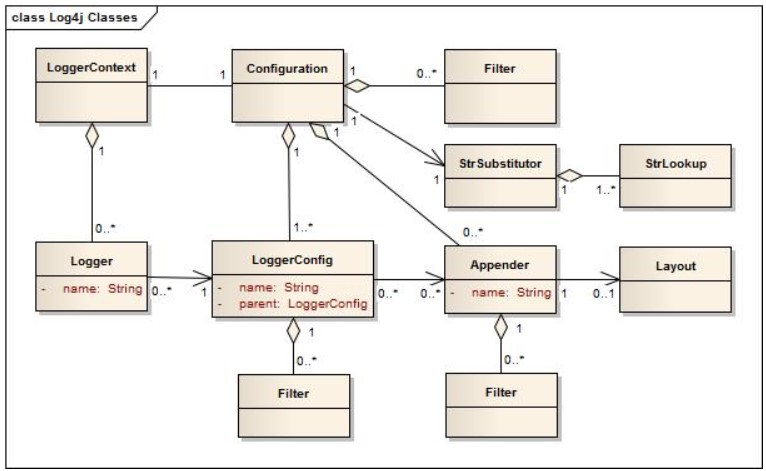
\includegraphics[scale=0.7]{pics/log4jArchitektur.jpg}
    \caption{log4J Architektur \cite{log4J}}
    \label{fig:impl:log4jArchitektur}
\end{figure}